% Created by tikzDevice version 0.7.0 on 2014-09-22 15:36:33
% !TEX encoding = UTF-8 Unicode
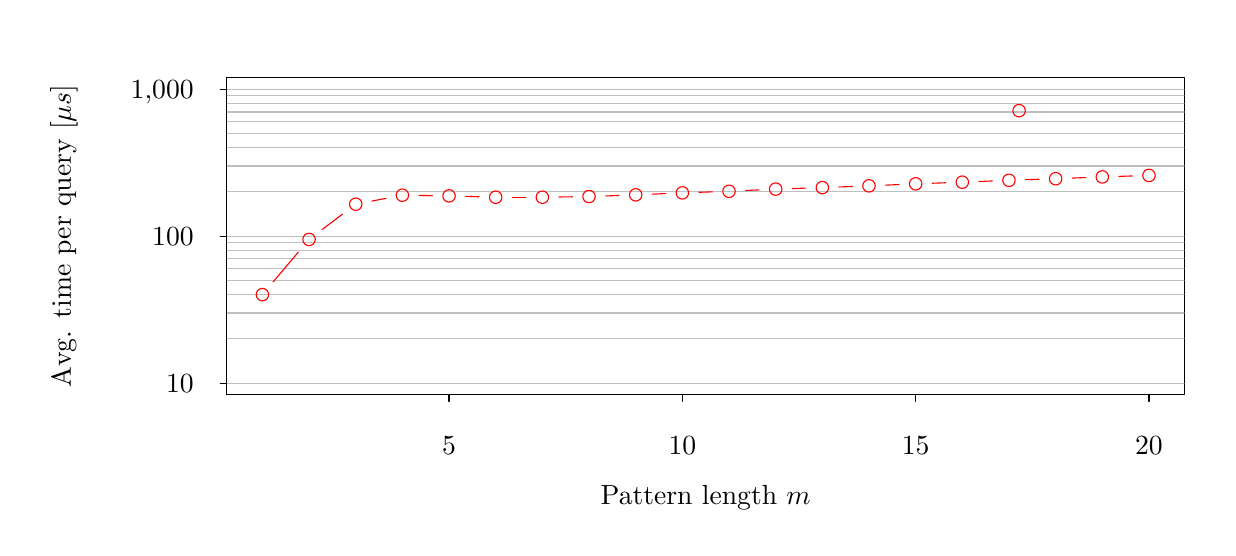
\begin{tikzpicture}[x=1pt,y=1pt]
\definecolor[named]{fillColor}{rgb}{1.00,1.00,1.00}
\path[use as bounding box,fill=fillColor,fill opacity=0.00] (0,0) rectangle (426.39,180.67);
\begin{scope}
\path[clip] (  0.00,  0.00) rectangle (426.39,180.67);
\definecolor[named]{drawColor}{rgb}{0.00,0.00,0.00}

\path[draw=drawColor,line width= 0.4pt,line join=round,line cap=round] (152.26, 48.00) -- (405.18, 48.00);

\path[draw=drawColor,line width= 0.4pt,line join=round,line cap=round] (152.26, 48.00) -- (152.26, 45.60);

\path[draw=drawColor,line width= 0.4pt,line join=round,line cap=round] (236.57, 48.00) -- (236.57, 45.60);

\path[draw=drawColor,line width= 0.4pt,line join=round,line cap=round] (320.87, 48.00) -- (320.87, 45.60);

\path[draw=drawColor,line width= 0.4pt,line join=round,line cap=round] (405.18, 48.00) -- (405.18, 45.60);

\node[text=drawColor,anchor=base,inner sep=0pt, outer sep=0pt, scale=  1.00] at (152.26, 26.40) {5};

\node[text=drawColor,anchor=base,inner sep=0pt, outer sep=0pt, scale=  1.00] at (236.57, 26.40) {10};

\node[text=drawColor,anchor=base,inner sep=0pt, outer sep=0pt, scale=  1.00] at (320.87, 26.40) {15};

\node[text=drawColor,anchor=base,inner sep=0pt, outer sep=0pt, scale=  1.00] at (405.18, 26.40) {20};

\path[draw=drawColor,line width= 0.4pt,line join=round,line cap=round] ( 72.00, 48.00) --
	(417.99, 48.00) --
	(417.99,162.67) --
	( 72.00,162.67) --
	( 72.00, 48.00);
\end{scope}
\begin{scope}
\path[clip] ( 48.00, 36.00) rectangle (423.99,180.67);
\definecolor[named]{drawColor}{rgb}{0.00,0.00,0.00}

\node[text=drawColor,anchor=base,inner sep=0pt, outer sep=0pt, scale=  1.20] at (245.00,167.53) {\bfseries \GOVII};

\node[text=drawColor,anchor=base,inner sep=0pt, outer sep=0pt, scale=  1.00] at (245.00,  2.40) {Pattern length};
\end{scope}
\begin{scope}
\path[clip] (  0.00,  0.00) rectangle (426.39,180.67);
\definecolor[named]{drawColor}{rgb}{0.00,0.00,0.00}

\node[text=drawColor,anchor=base,inner sep=0pt, outer sep=0pt, scale=  1.00] at (245.00,  8.40) {Pattern length $m$};

\node[text=drawColor,rotate= 90.00,anchor=base,inner sep=0pt, outer sep=0pt, scale=  1.00] at ( 15.60,105.34) {Avg. time per query [$\mu s$]};

\path[draw=drawColor,line width= 0.4pt,line join=round,line cap=round] ( 72.00, 52.25) -- ( 72.00,162.68);

\path[draw=drawColor,line width= 0.4pt,line join=round,line cap=round] ( 72.00, 52.25) -- ( 69.60, 52.25);

\path[draw=drawColor,line width= 0.4pt,line join=round,line cap=round] ( 72.00,105.34) -- ( 69.60,105.34);

\path[draw=drawColor,line width= 0.4pt,line join=round,line cap=round] ( 72.00,158.43) -- ( 69.60,158.43);

\node[text=drawColor,anchor=base east,inner sep=0pt, outer sep=0pt, scale=  1.00] at ( 60.00, 48.80) {10};

\node[text=drawColor,anchor=base east,inner sep=0pt, outer sep=0pt, scale=  1.00] at ( 60.00,101.89) {100};

\node[text=drawColor,anchor=base east,inner sep=0pt, outer sep=0pt, scale=  1.00] at ( 60.00,154.98) {1,000};
\end{scope}
\begin{scope}
\path[clip] ( 72.00, 48.00) rectangle (417.99,162.67);
\definecolor[named]{drawColor}{rgb}{0.75,0.75,0.75}

\path[draw=drawColor,line width= 0.4pt,line join=round,line cap=round] ( 72.00, 52.25) -- (417.99, 52.25);

\path[draw=drawColor,line width= 0.4pt,line join=round,line cap=round] ( 72.00, 68.23) -- (417.99, 68.23);

\path[draw=drawColor,line width= 0.4pt,line join=round,line cap=round] ( 72.00, 77.58) -- (417.99, 77.58);

\path[draw=drawColor,line width= 0.4pt,line join=round,line cap=round] ( 72.00, 84.21) -- (417.99, 84.21);

\path[draw=drawColor,line width= 0.4pt,line join=round,line cap=round] ( 72.00, 89.36) -- (417.99, 89.36);

\path[draw=drawColor,line width= 0.4pt,line join=round,line cap=round] ( 72.00, 93.56) -- (417.99, 93.56);

\path[draw=drawColor,line width= 0.4pt,line join=round,line cap=round] ( 72.00, 97.11) -- (417.99, 97.11);

\path[draw=drawColor,line width= 0.4pt,line join=round,line cap=round] ( 72.00,100.19) -- (417.99,100.19);

\path[draw=drawColor,line width= 0.4pt,line join=round,line cap=round] ( 72.00,102.91) -- (417.99,102.91);

\path[draw=drawColor,line width= 0.4pt,line join=round,line cap=round] ( 72.00,105.34) -- (417.99,105.34);

\path[draw=drawColor,line width= 0.4pt,line join=round,line cap=round] ( 72.00,121.32) -- (417.99,121.32);

\path[draw=drawColor,line width= 0.4pt,line join=round,line cap=round] ( 72.00,130.67) -- (417.99,130.67);

\path[draw=drawColor,line width= 0.4pt,line join=round,line cap=round] ( 72.00,137.30) -- (417.99,137.30);

\path[draw=drawColor,line width= 0.4pt,line join=round,line cap=round] ( 72.00,142.45) -- (417.99,142.45);

\path[draw=drawColor,line width= 0.4pt,line join=round,line cap=round] ( 72.00,146.65) -- (417.99,146.65);

\path[draw=drawColor,line width= 0.4pt,line join=round,line cap=round] ( 72.00,150.20) -- (417.99,150.20);

\path[draw=drawColor,line width= 0.4pt,line join=round,line cap=round] ( 72.00,153.28) -- (417.99,153.28);

\path[draw=drawColor,line width= 0.4pt,line join=round,line cap=round] ( 72.00,156.00) -- (417.99,156.00);

\path[draw=drawColor,line width= 0.4pt,line join=round,line cap=round] ( 72.00,158.43) -- (417.99,158.43);

\path[draw=drawColor,line width= 0.4pt,line join=round,line cap=round] ( 72.00,174.41) -- (417.99,174.41);
\definecolor[named]{drawColor}{rgb}{1.00,0.00,0.00}

\path[draw=drawColor,line width= 0.4pt,line join=round,line cap=round] ( 88.69, 88.79) -- ( 97.80, 99.57);

\path[draw=drawColor,line width= 0.4pt,line join=round,line cap=round] (106.46,107.77) -- (113.75,113.27);

\path[draw=drawColor,line width= 0.4pt,line join=round,line cap=round] (124.43,118.02) -- (129.51,119.00);

\path[draw=drawColor,line width= 0.4pt,line join=round,line cap=round] (141.40,120.05) -- (146.26,119.98);

\path[draw=drawColor,line width= 0.4pt,line join=round,line cap=round] (158.26,119.72) -- (163.12,119.57);

\path[draw=drawColor,line width= 0.4pt,line join=round,line cap=round] (175.12,119.40) -- (179.98,119.40);

\path[draw=drawColor,line width= 0.4pt,line join=round,line cap=round] (191.98,119.49) -- (196.84,119.56);

\path[draw=drawColor,line width= 0.4pt,line join=round,line cap=round] (208.84,119.86) -- (213.71,120.04);

\path[draw=drawColor,line width= 0.4pt,line join=round,line cap=round] (225.70,120.51) -- (230.57,120.72);

\path[draw=drawColor,line width= 0.4pt,line join=round,line cap=round] (242.56,121.18) -- (247.43,121.34);

\path[draw=drawColor,line width= 0.4pt,line join=round,line cap=round] (259.42,121.83) -- (264.29,122.05);

\path[draw=drawColor,line width= 0.4pt,line join=round,line cap=round] (276.29,122.53) -- (281.15,122.69);

\path[draw=drawColor,line width= 0.4pt,line join=round,line cap=round] (293.15,123.11) -- (298.02,123.29);

\path[draw=drawColor,line width= 0.4pt,line join=round,line cap=round] (310.01,123.77) -- (314.88,123.98);

\path[draw=drawColor,line width= 0.4pt,line join=round,line cap=round] (326.87,124.45) -- (331.74,124.63);

\path[draw=drawColor,line width= 0.4pt,line join=round,line cap=round] (343.73,125.08) -- (348.60,125.28);

\path[draw=drawColor,line width= 0.4pt,line join=round,line cap=round] (360.59,125.73) -- (365.46,125.89);

\path[draw=drawColor,line width= 0.4pt,line join=round,line cap=round] (377.45,126.32) -- (382.32,126.51);

\path[draw=drawColor,line width= 0.4pt,line join=round,line cap=round] (394.31,126.93) -- (399.18,127.09);

\path[draw=drawColor,line width= 0.4pt,line join=round,line cap=round] ( 84.81, 84.21) circle (  2.25);

\path[draw=drawColor,line width= 0.4pt,line join=round,line cap=round] (101.68,104.15) circle (  2.25);

\path[draw=drawColor,line width= 0.4pt,line join=round,line cap=round] (118.54,116.88) circle (  2.25);

\path[draw=drawColor,line width= 0.4pt,line join=round,line cap=round] (135.40,120.14) circle (  2.25);

\path[draw=drawColor,line width= 0.4pt,line join=round,line cap=round] (152.26,119.89) circle (  2.25);

\path[draw=drawColor,line width= 0.4pt,line join=round,line cap=round] (169.12,119.40) circle (  2.25);

\path[draw=drawColor,line width= 0.4pt,line join=round,line cap=round] (185.98,119.40) circle (  2.25);

\path[draw=drawColor,line width= 0.4pt,line join=round,line cap=round] (202.84,119.65) circle (  2.25);

\path[draw=drawColor,line width= 0.4pt,line join=round,line cap=round] (219.70,120.26) circle (  2.25);

\path[draw=drawColor,line width= 0.4pt,line join=round,line cap=round] (236.57,120.97) circle (  2.25);

\path[draw=drawColor,line width= 0.4pt,line join=round,line cap=round] (253.43,121.55) circle (  2.25);

\path[draw=drawColor,line width= 0.4pt,line join=round,line cap=round] (270.29,122.33) circle (  2.25);

\path[draw=drawColor,line width= 0.4pt,line join=round,line cap=round] (287.15,122.88) circle (  2.25);

\path[draw=drawColor,line width= 0.4pt,line join=round,line cap=round] (304.01,123.52) circle (  2.25);

\path[draw=drawColor,line width= 0.4pt,line join=round,line cap=round] (320.87,124.24) circle (  2.25);

\path[draw=drawColor,line width= 0.4pt,line join=round,line cap=round] (337.73,124.84) circle (  2.25);

\path[draw=drawColor,line width= 0.4pt,line join=round,line cap=round] (354.59,125.52) circle (  2.25);

\path[draw=drawColor,line width= 0.4pt,line join=round,line cap=round] (371.46,126.09) circle (  2.25);

\path[draw=drawColor,line width= 0.4pt,line join=round,line cap=round] (388.32,126.74) circle (  2.25);

\path[draw=drawColor,line width= 0.4pt,line join=round,line cap=round] (405.18,127.28) circle (  2.25);

\path[draw=drawColor,line width= 0.4pt,line join=round,line cap=round] (358.25,150.68) circle (  2.25);
\definecolor[named]{drawColor}{rgb}{0.00,0.00,0.00}

\node[text=drawColor,anchor=base west,inner sep=0pt, outer sep=0pt, scale=  1.00] at (367.25,147.23) {\IDXNNX};
\end{scope}
\end{tikzpicture}
